%   Filename    : appendix_C.tex

\chapter{Complete Feature Correlation Analysis}
\label{app:correlation}

This appendix provides the complete feature correlation analysis for the extracted variables used in the study. The larger heatmap shown here complements the reduced version presented in Chapter~4 and allows clearer inspection of relationships within and across feature families, including supplementary alignment features, clipping-based features, k-mer features, microhomology features, and other alignment-related variables.

Figure~\ref{fig:app_correlation_heatmap_full} presents the full correlation heatmap for all extracted features. Overall, alignment-derived and clipping-related variables form the most visible correlated cluster, while k-mer and microhomology features remain comparatively independent from most other feature groups.

\begin{figure}[H]
\centering
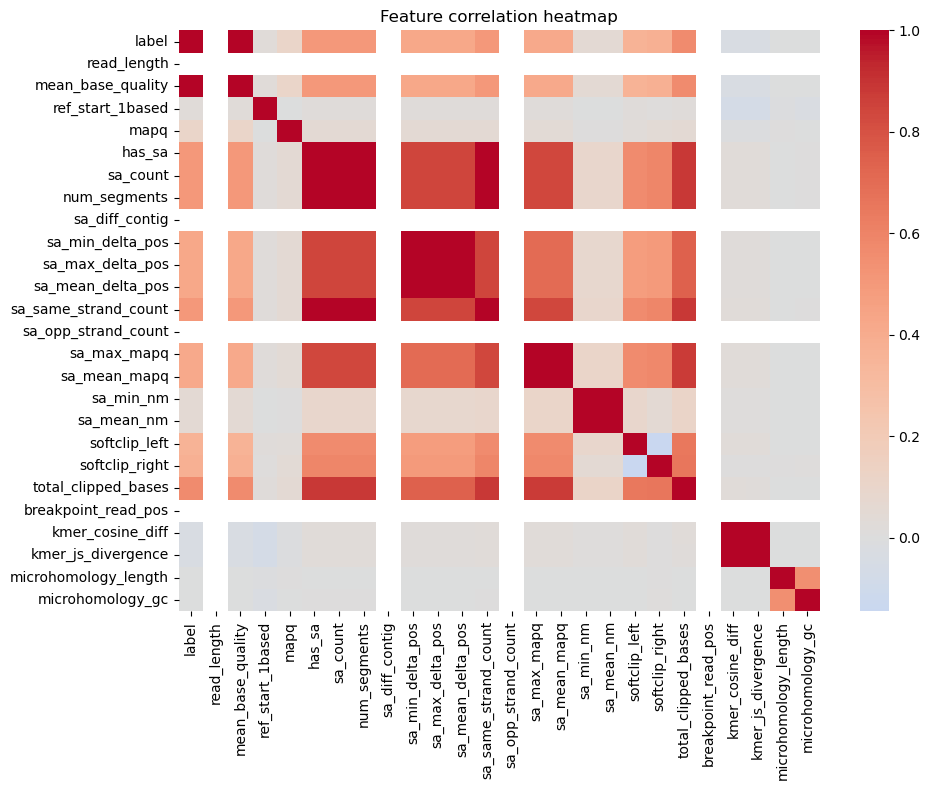
\includegraphics[width=0.9\textwidth]{../notebooks/figures/correlation.png}
\caption{Complete feature correlation heatmap for all extracted variables.}
\label{fig:app_correlation_heatmap_full}
\end{figure}

\FloatBarrier